 \taskpic{ Говорят, что в архиве Снеллиуса нашли рисунок с оптической
   схемой. От времени чернила выцвели, и на бумаге остались видны
   только предмет и его изображение, даваемое тонкой линзой.\\
   1) восстановите построением по имеющимся данным положение линзы.\\
   2) найдите положение фокусов линзы.  \\
   3) можно ли, исходя из рисунка, сказать, какая (собирающая или
   рассеивающая) была линза?  }{
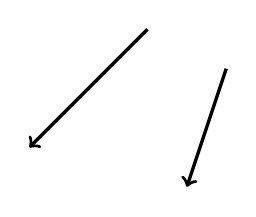
\begin{tikzpicture}
  \draw[very thick,->] (2,3) -- (0.5,1.5);
  \draw[very thick,->] (3,2.5) -- (2.5,1);
\end{tikzpicture}
}